\newpage
\section{Teknisk Verkemåte}
\thispagestyle{fancy}
Sandre reinseanlegg er konstruert basert på SBR-teknologi

\gls{SBR} står for 'Sequence Batch Reactor', på norsk 'sekvensiell batchreaktor'.\newline
\gls{SBR} er en reinsemetode der alle prosessar føregår i same reaktortank. 
Reaktor nyttar biologisk reinsing, ved hjelp av akktivert slam som inneheld mikroorganismar, for å koagulere 
og fjerne løyste og ikkje sedimenterbare partiklar samt stabilisere organisk materiale. 
Avløpsvatn tilførast reaktor i 'batcher' for å bli reinsa og uttappa. 
Kvar avløps-batch går igjennom ein reaktorsekvens som består av følgande fem delsekvensar.
\newline

\begin{figure}[htbp]
    \centering
    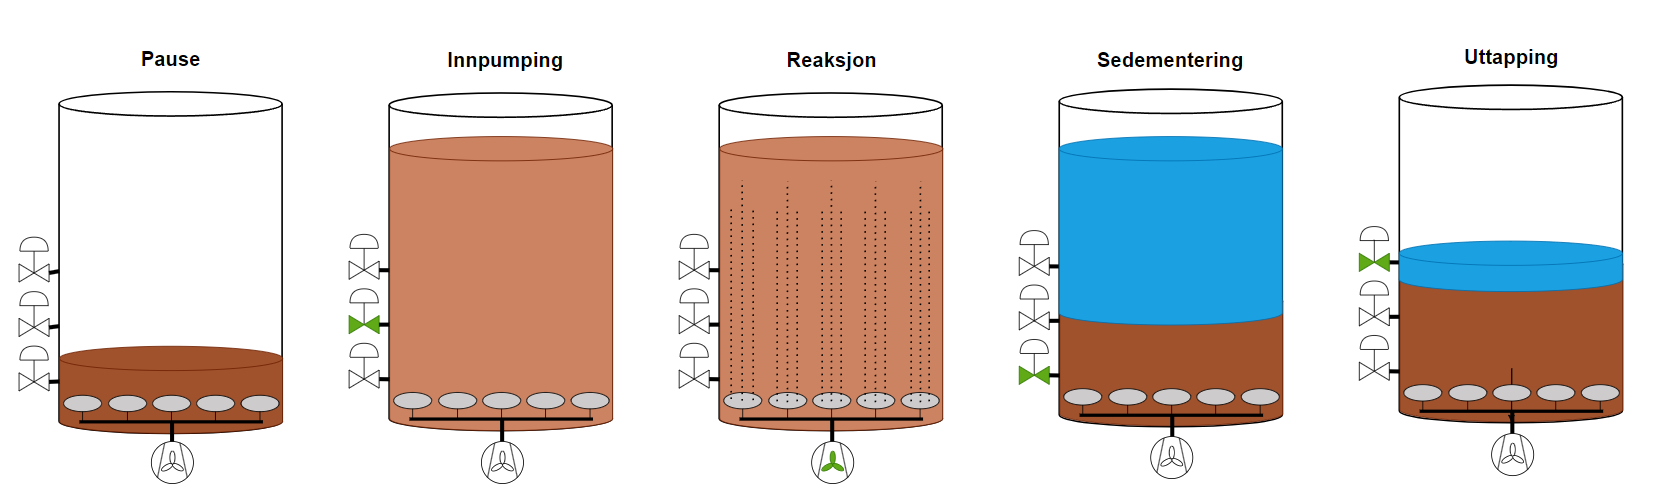
\includegraphics[width=1\textwidth]{Figurar/SBR-V2.png}
    \caption{\gls{SBR}-prossessen}\label{fig:SBR-Prosessen}
\end{figure}


\begin{enumerate}
    \item \textbf{\makebox[3cm][l]{Pause}:} Reaktoren venter til det er behov for dens kapasitet.
    \item \textbf{\makebox[3cm][l]{Innpumping}:} Reaktoren mottar avlaupsvatn, normalt ifrå ein utjamningstank.
    \item \textbf{\makebox[3cm][l]{Reaksjon}:} Reaktoren periodisk luftast for å tilføre oksygen til mikroorganismane.
    \item \textbf{\makebox[3cm][l]{Sedementering}:} Reaktoren sedementerer ved hjelp av gravitasjon. Overskudd slam fjernast.
    \item \textbf{\makebox[3cm][l]{Uttapping}:} Reaktoren drenerar reisa vatn mot resepient.
\end{enumerate}

Meir detaljert informasjon om \gls{SBR} og anleggets teknolgiske prinsipp er tilgjengeleg i anleggets
funksjonsbeskrivelse. (INSERT APPENDIX REFERANSE MED LINK)

